\documentclass[authoryear, review, 11pt]{elsarticle}

\setlength{\textwidth}{6.5in}
%\setlength{\textheight}{9in}
\setlength{\topmargin}{0in}
\setlength{\oddsidemargin}{0in}
\setlength{\evensidemargin}{0in}

\usepackage{amsmath}
\usepackage{amsthm}
\usepackage{amssymb}
\usepackage{mathabx}
\usepackage{bm}
\usepackage{multirow}

%\geometry{landscape}                % Activate for for rotated page geometry
\usepackage[parfill]{parskip}    % Activate to begin paragraphs with an empty line rather than an indent
\usepackage{graphicx}
\usepackage{epstopdf}
\usepackage{natbib}
\usepackage{verbatim}

\usepackage{endfloat}

\usepackage{relsize}
\usepackage{caption}
\usepackage{subcaption}
%\usepackage{fullpage}
\usepackage{booktabs}

\DeclareGraphicsRule{.tif}{png}{.png}{`convert #1 `dirname #1`/`basename #1 .tif`.png}
\DeclareMathOperator*{\argmin}{\arg\!\min}
\DeclareMathOperator*{\argmax}{\arg\!\max}
\DeclareMathOperator*{\bw}{\mbox{bw}}
\DeclareMathOperator*{\df}{\mbox{df}}
\newcommand{\vect}[1]{\bm{#1}}
\newcommand{\E}{\mathop{\mathbb E}}


\title{Modeling PalEON biomass}
\author{Wesley Brooks}
\date{}                                           % Activate to display a given date or no date

\begin{document}
\maketitle
%\section{}
%\subsection{}


\section{Introduction}
Our objective is a  model of the biomass of each species in each grid cell, where the only parameters used to calibrate the models are location and species composition. It is important to come up with an estimated probability that a given cell will have no biomass of a given species, and also to model the variance of the biomass estimate.\\


\section{Philosophy}
Consider twi different kinds of errors:

\begin{itemize}
  \item Natural variability in biomass (noise)
  \item Measurement error
\end{itemize}

Jun and I discussed the interpretation of a model for biomass. At the time I saw the effort being directed toward getting a model that tells us, based on our survey of the forests at time of settlement, how much biomass there was on the landscape at time of settlement. On the other hand, Jun says that the goal is to model the process that gives rise to biomass on the landscape, observed through the survey at time of settlement.\\

As a practical matter, one implication is that grid cells where there were small but nonzero biomass observations are treated differently. In my view, the fact that, say, a spruce tree was seen in grid cell 517 is enough to say that there is zero probability of there being no spruce biomass in cell 517. In Jun's view, we could easily imagine the same process populating the landscape in such a way that, randomly, cell 517 has no spruce trees. So there's a positive probability of zero spruce in cell 517.\\

If measurement error was the only possible error, then it we could say that observing even a single spruce tree in a cell means that spruce biomass is nonzero in that cell. But since there is also random noise, observing a spruce tree doesn't guarantee that spruce biomass will be nonzero the next day or year or whenever...\\


\section{Chris' proposal}
Chris proposed the following:\*
Let $Y_{k,s}$ denote the biomass of taxon $k$ in grid cell $s$. Let $n_s$ be the number of PLS survey points within cell $s$, and note that two trees are sampled at each survey point. Then, letting $\hat{\lambda}_{s,i}$ be the estimate for total stem density (i.e. taxa are aggregated) at survey point $s_i$, $d_{s,i,j}$ the measured DBH for tree $j$ at survey point $s_i$, and $\left(a_k, b_k\right)$ allometric parameters for taxon $k$, the biomass measurement for taxon $k$ in grid cell $s$ is:\*
\begin{equation*}
  \begin{split}
    Y_{k,s} &= \left[ n_s \right]^{-1} \sum\limits_{i=1}^{n_s} \hat{\lambda}_{s,i} \sum\limits_{j=1}^{2} 2^{-1} a_k d_{s,i,j}^{b_k} I(\text{tree}_{s,i,j} \text{ is in taxon }k)\\
    &= \left[ 2 \cdot n_s \right]^{-1} \sum\limits_{i=1}^{n_s} \hat{\lambda}_{s,i} \sum\limits_{j=1}^{2} h_k(d_{s,i,j}) A_{s,i,j}(k)
  \end{split}
\end{equation*}
Where $h_k(\cdot)$ is the allometric equation for taxon $k$ and $A_{s,i,j}(k)$ is is the indicator of the event that $\text{tree}_{s,i,j}$ is in taxon $k$.\\

Now we want to use these measurement of biomass as the observations on which a model of biomass will be based. For this, Chris proposes a log-normal model for $Y_{k,s}$ based on taxon $k$'s composition fraction, $p_k(s)$:\*
\begin{equation*}
  \begin{split}
    \log Y_{k,s} &\sim \mathcal{N}\left(g_k(s), \hat{V}_{k,s}\right)\\
    g_k(s) &\sim \text{GP}\left(f(p_k(s)), \Sigma \right)
  \end{split}
\end{equation*}
That is, the Gaussian process $g_k(\cdot)$ sets the mean for a log-normal model of $Y_{k,s}$. The variance components are $\Sigma$, which is a spatial covariance, and $V_{k,s}$, which is random noise.\\


\section{First look}
Consider the `Oaks' taxon. In Figure \ref{fig:oaks-biomass-observed}, the log of oak biomass is plotted on a heatmap. \\


\section{Models}


There are two possible directions here: a two-stage hierarchical model, where in stage one we randomly decide whether a given cell has nonzero biomass, and then if so stage two randomly sets the biomass; alternatively, a single-stage model with zero-inflation, maybe one that could be tuned like a \verb!glm! (e.g. a Tweedie model).\\


\subsection{Two-stage model}
The two-stage model (sometimes called the delta approach) has one stage for determining the probability that a given species has zero biomass in a cell and another stage for estimating the distribution of biomass, given that it is nonzero. Since in the observed data there is an almost perfect correspondence between cells where biomass is zero and cells where composition is zero, the first stage of the model needs to look at the composition of neighboring cells:\*
\begin{equation*}
  \begin{split}
    B_{k,s} &\sim \text{Bernoulli}(\mu_{s,k})\\
    \mu_{s, k} &= \alpha_{s,k} + \sum\limits_{i \in \mathcal{N}_s} \beta p_k(s)
  \end{split}
\end{equation*}

Note that the composition is currently an observation, not a model. Since composition fraction is zero if and only if the biomass is zero, this cell's composition fraction is not a useful variable in modeling its probability of zero biomass. Instead, we use the mean composition fraction across the first-order neighborhood.


\subsection{Single-stage (Tweedie model)}
Tweedie family of distributions for $\theta \in (0,1)$:\\
\begin{equation*}
  \begin{split}
    N &\sim \text{Poisson}(\lambda)    \\
    Z_i &\sim \text{Gamma}(\alpha, \tau)    \\
    Y &= \sum\limits_{i=1}^N Z_i \\
    \lambda &= \phi^{-1} \frac{\mu^{2-\theta}}{2-\theta} \\
    \alpha &= \frac{2-\theta}{\theta-1} \\
    \tau &= \phi (\theta - 1) \mu^{\theta - 1}    \\
    \eta(s) &= f\left(\bm{x}(s)\right) = g\left(\mu(s)\right)\\
    \mu(s) &= g^{-1}\left(\eta(s)\right)
  \end{split}
\end{equation*}

Where $g(\cdot)$ is the link function, $\bm{x}(s)$ is the vector of covariates ($x, y$ coordinates and composition fraction) at location $s$.

The variance function of a Tweedie model is
\[
  V(\mu)  = \phi^{-1} \frac{\mu^{2-p}}{2-p}
\]

So it may be possible to select the power parameter $p$ based on the shape of the deviance residuals (i.e. the location-scale plot of the deviance residuals). The deviance residuals should have constant variance, so $p$ was selected to acheive that goal (see Figure \ref{fig:oaks-tweedie2-location-scale}).

\section{Figures}
\begin{figure}
	\begin{center}
	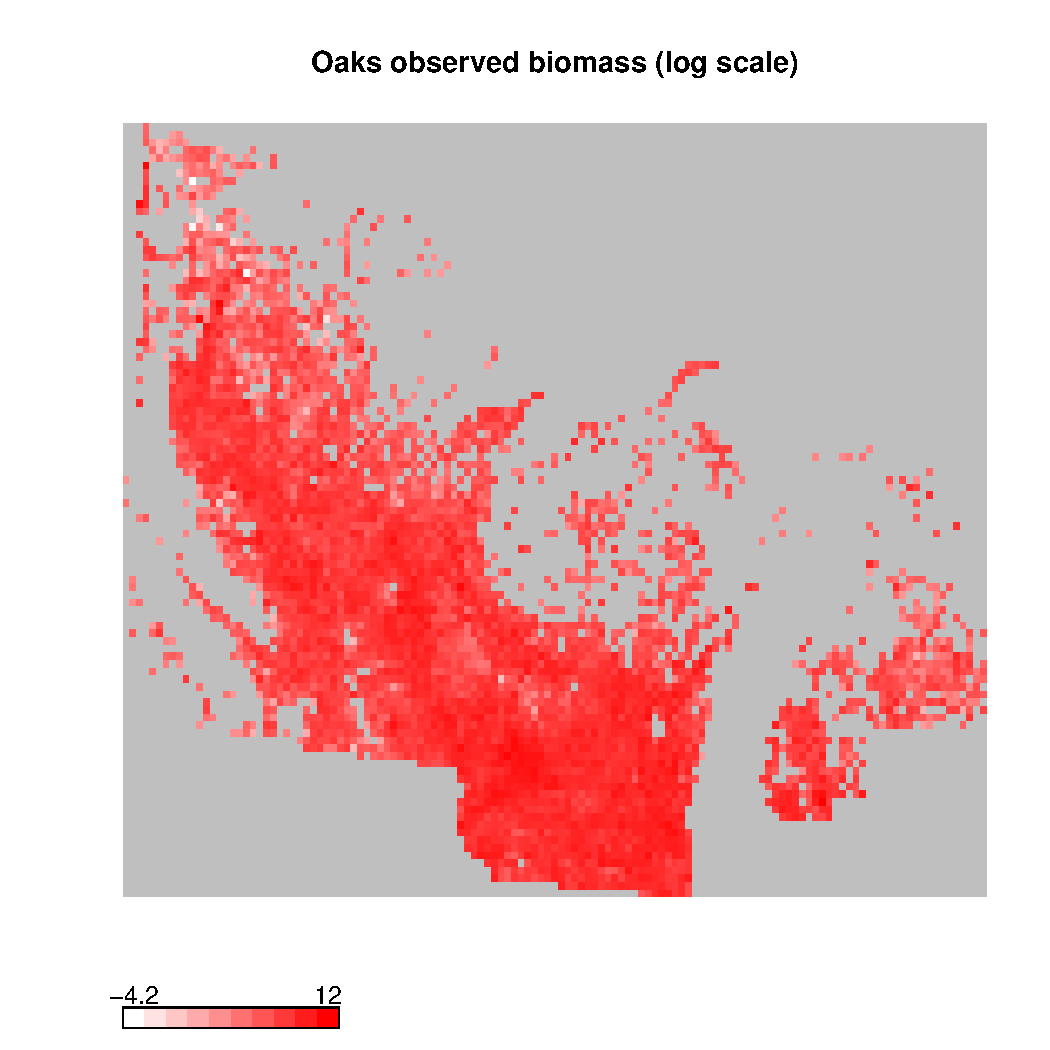
\includegraphics[width=5in]{../../figures//Oaks-biomass-observed.pdf}
	\caption{\label{fig:oaks-biomass-observed}}
	\end{center}
\end{figure}

\begin{figure}
	\begin{center}
	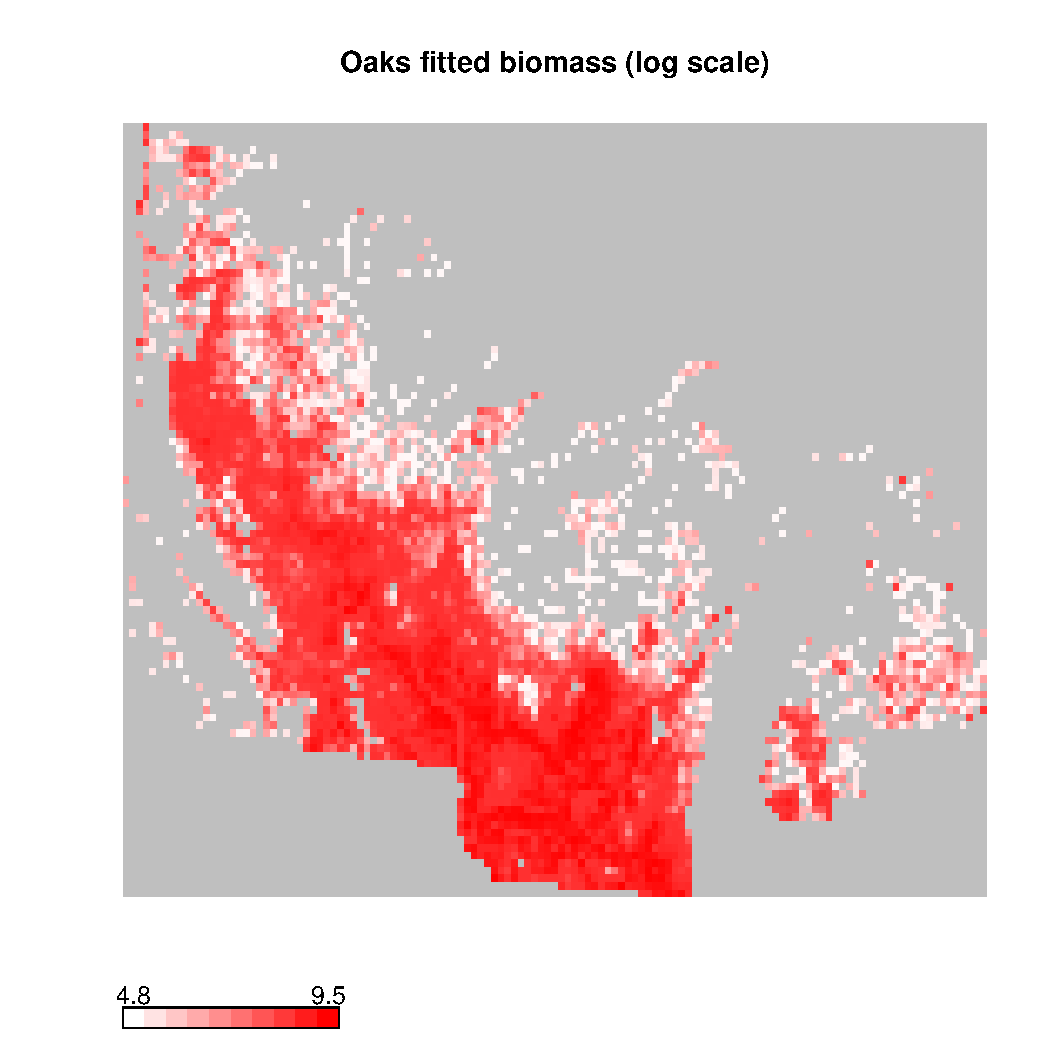
\includegraphics[width=5in]{../../figures/Oaks-biomass-fitted.pdf}
	\caption{\label{fig:oaks-biomass-fitted}}
	\end{center}
\end{figure}

\begin{figure}
	\begin{center}
	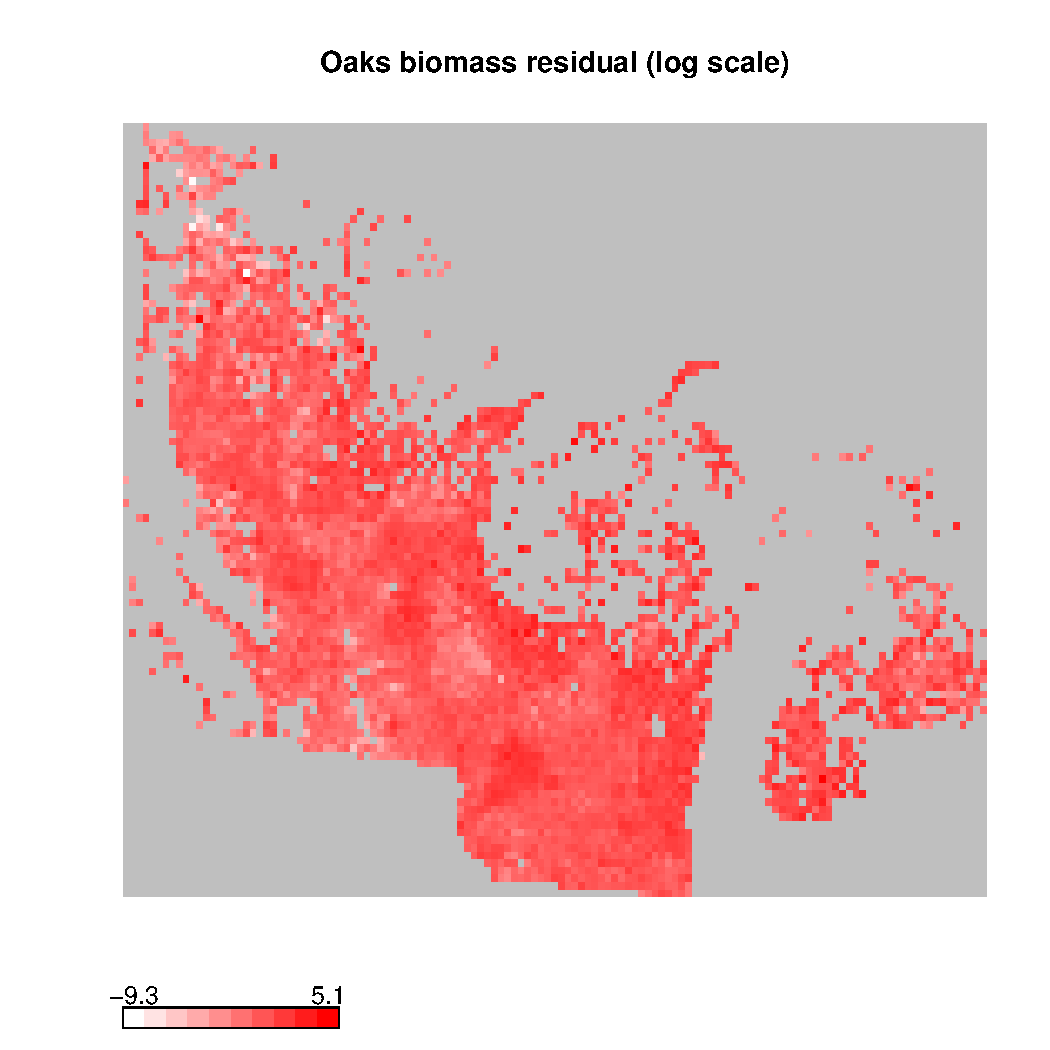
\includegraphics[width=5in]{../../figures/Oaks-biomass-residual.pdf}
	\caption{\label{fig:oaks-biomass-residual}}
	\end{center}
\end{figure}

\begin{figure}
	\begin{center}
	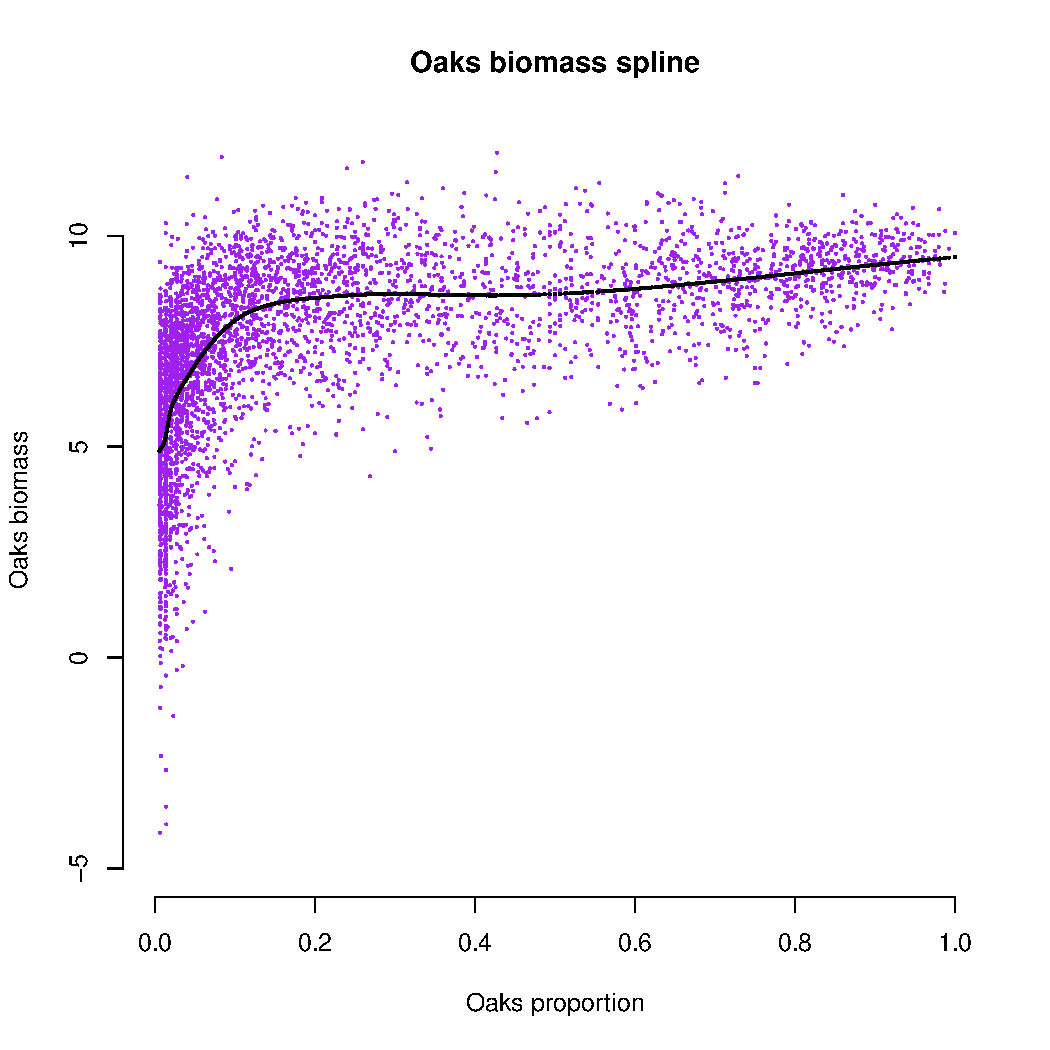
\includegraphics[width=5in]{../../figures/Exploration/Oaks-biomass-spline.pdf}
	\caption{\label{fig:oaks-biomass-spline}}
	\end{center}
\end{figure}



\begin{figure}
	\begin{center}
	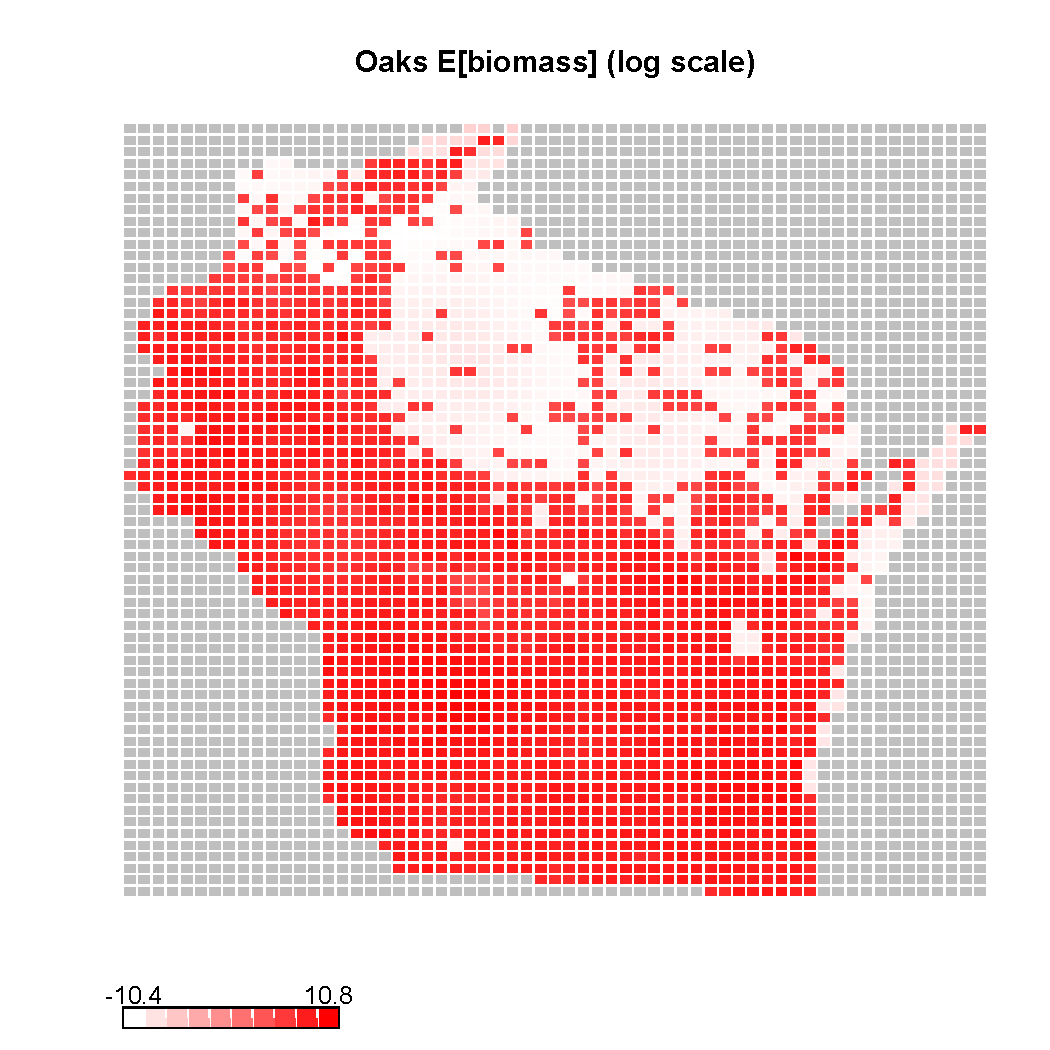
\includegraphics[width=5in]{../../figures/Exploration/Oak-Tweedie-E-biomass.pdf}
	\caption{\label{fig:oaks-biomass-observed}}
	\end{center}
\end{figure}

\begin{figure}
	\begin{center}
	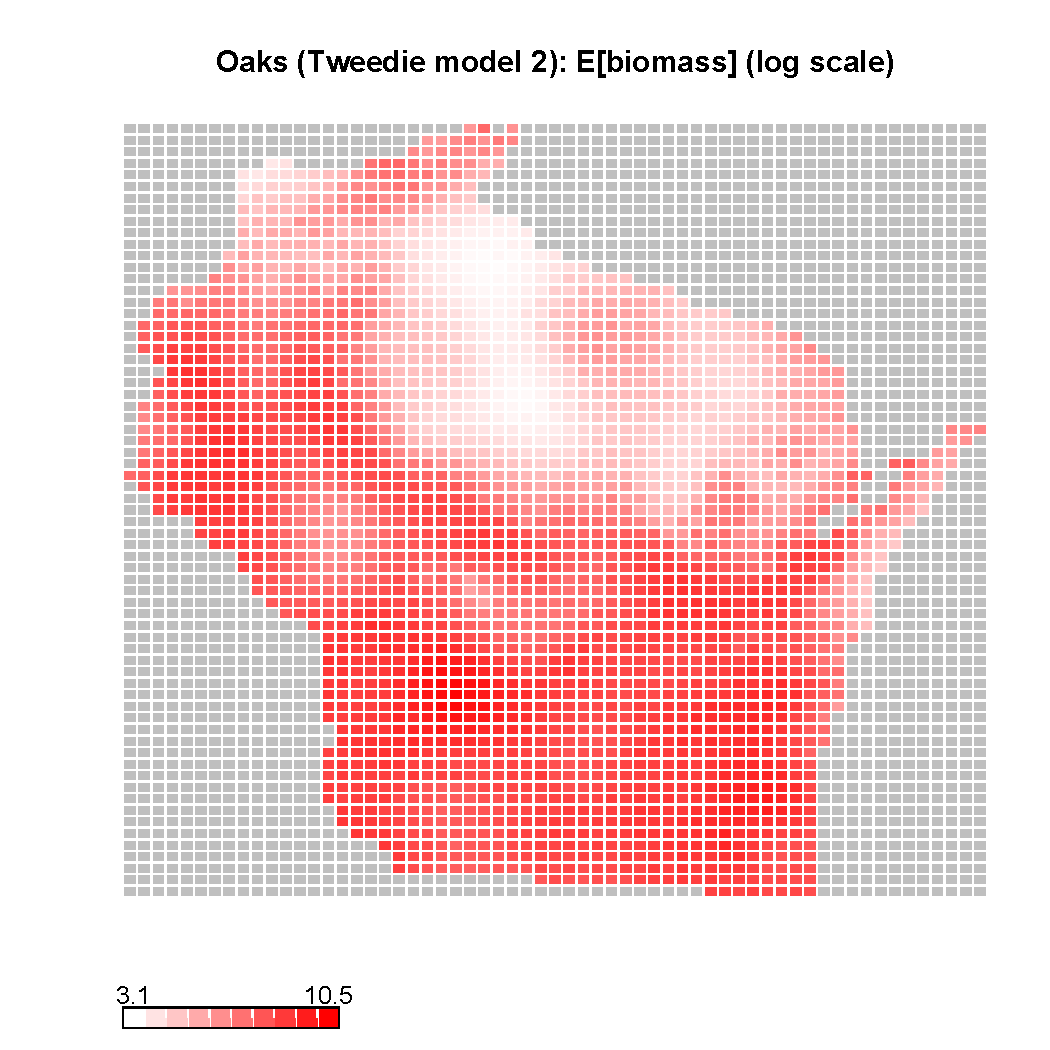
\includegraphics[width=5in]{../../figures/Exploration/Oak-Tweedie2-E-biomass.pdf}
	\caption{\label{fig:oaks-biomass-fitted}}
	\end{center}
\end{figure}

\begin{figure}
	\begin{center}
	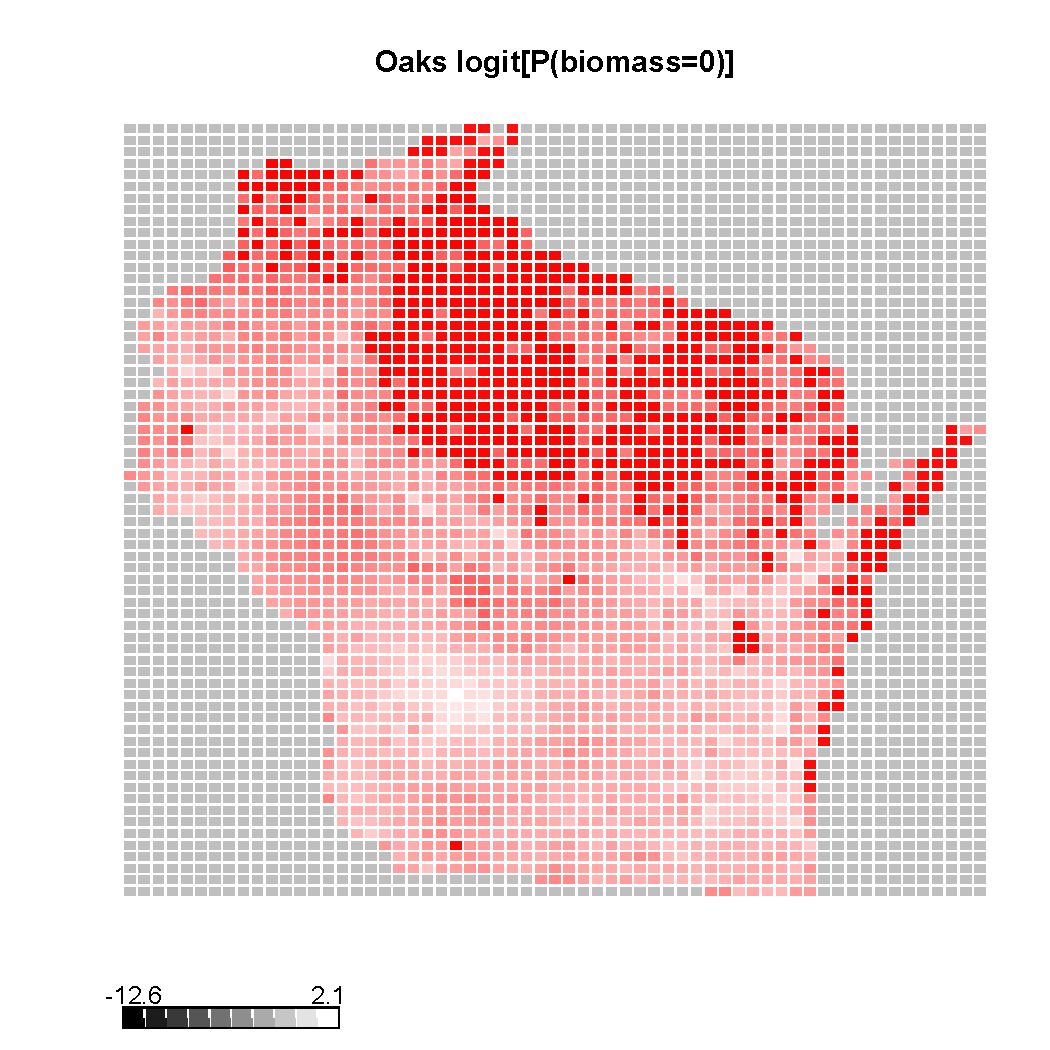
\includegraphics[width=5in]{../../figures/Exploration/Oak-Tweedie-P0-biomass.pdf}
	\caption{\label{fig:oaks-biomass-residual}}
	\end{center}
\end{figure}

\begin{figure}
	\begin{center}
	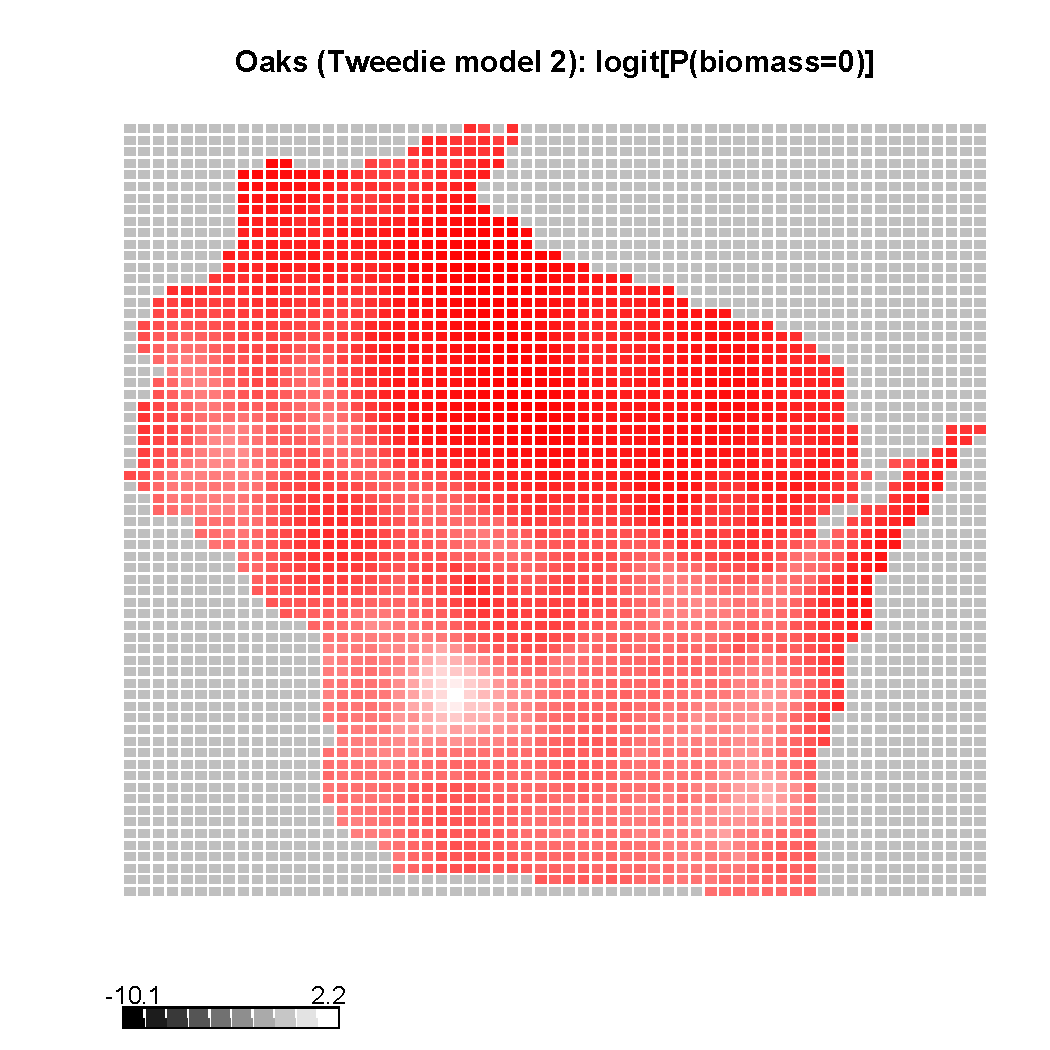
\includegraphics[width=5in]{../../figures/Exploration/Oak-Tweedie2-P0-biomass.pdf}
	\caption{\label{fig:oaks-biomass-spline}}
	\end{center}
\end{figure}

\begin{figure}
	\begin{center}
	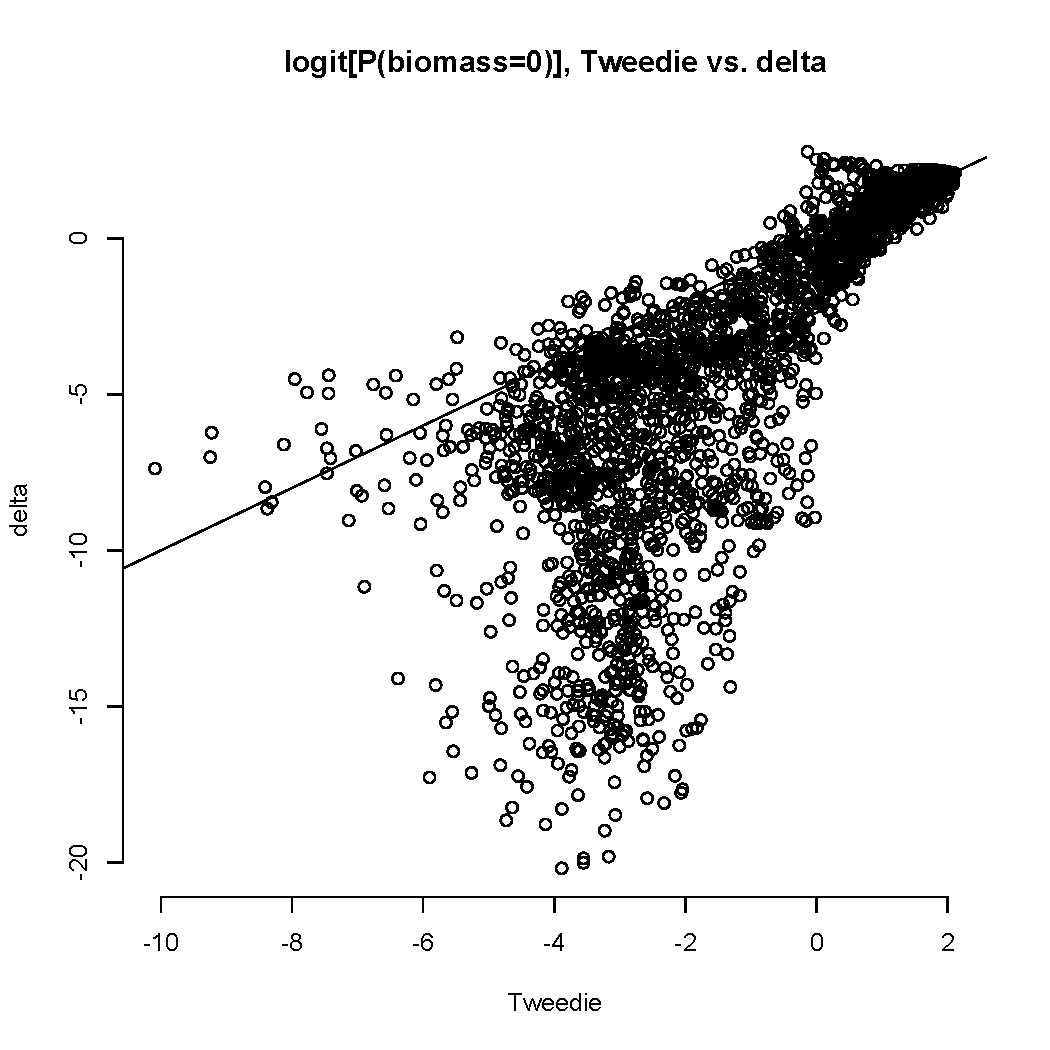
\includegraphics[width=5in]{../../figures/Exploration/Oak-P0-biomass-tweedie2-v-delta.pdf}
	\caption{\label{fig:oaks-biomass-spline}}
	\end{center}
\end{figure}

\begin{figure}
	\begin{center}
	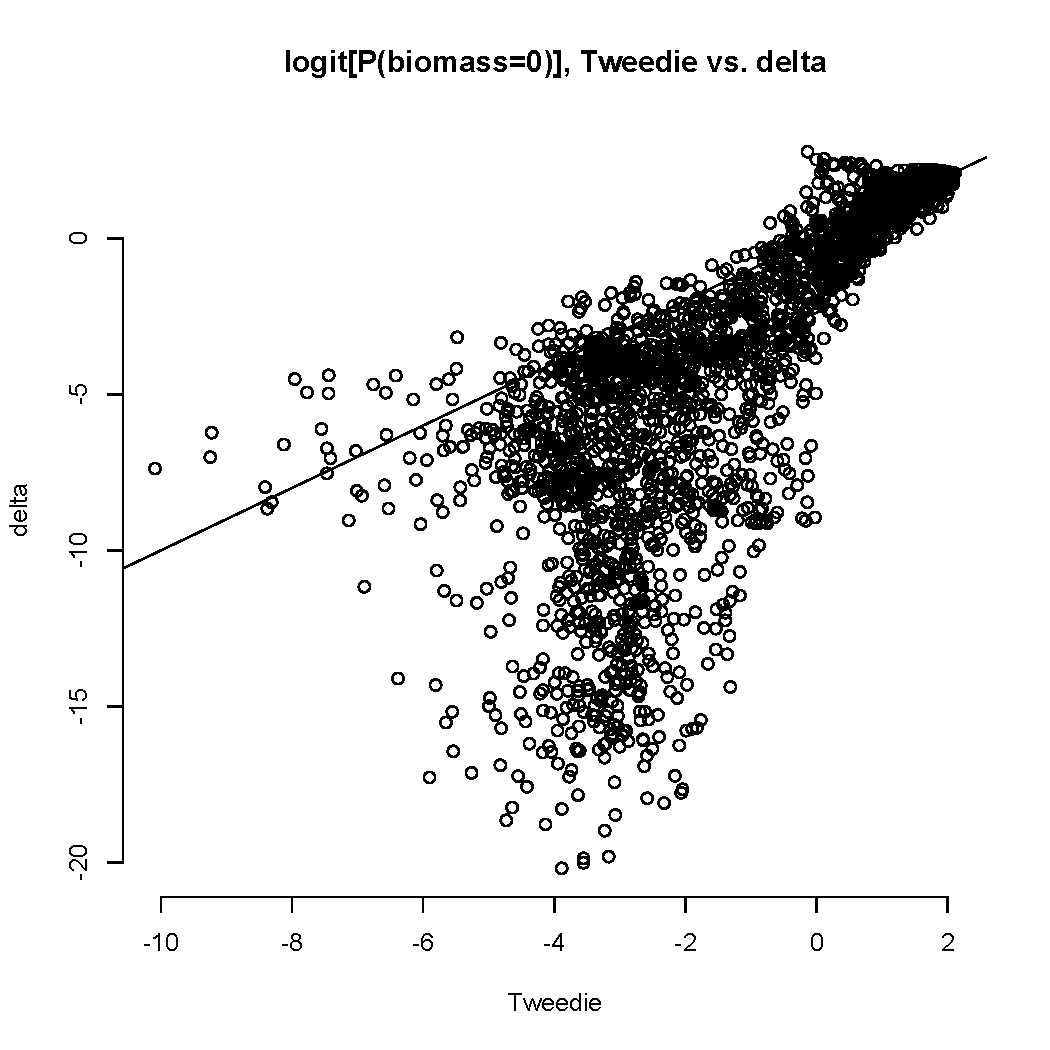
\includegraphics[width=5in]{../../figures/Exploration/Oak-P0-biomass-tweedie2-v-delta.pdf}
	\caption{\label{fig:oaks-biomass-spline}}
	\end{center}
\end{figure}


\begin{figure}
	\begin{center}
	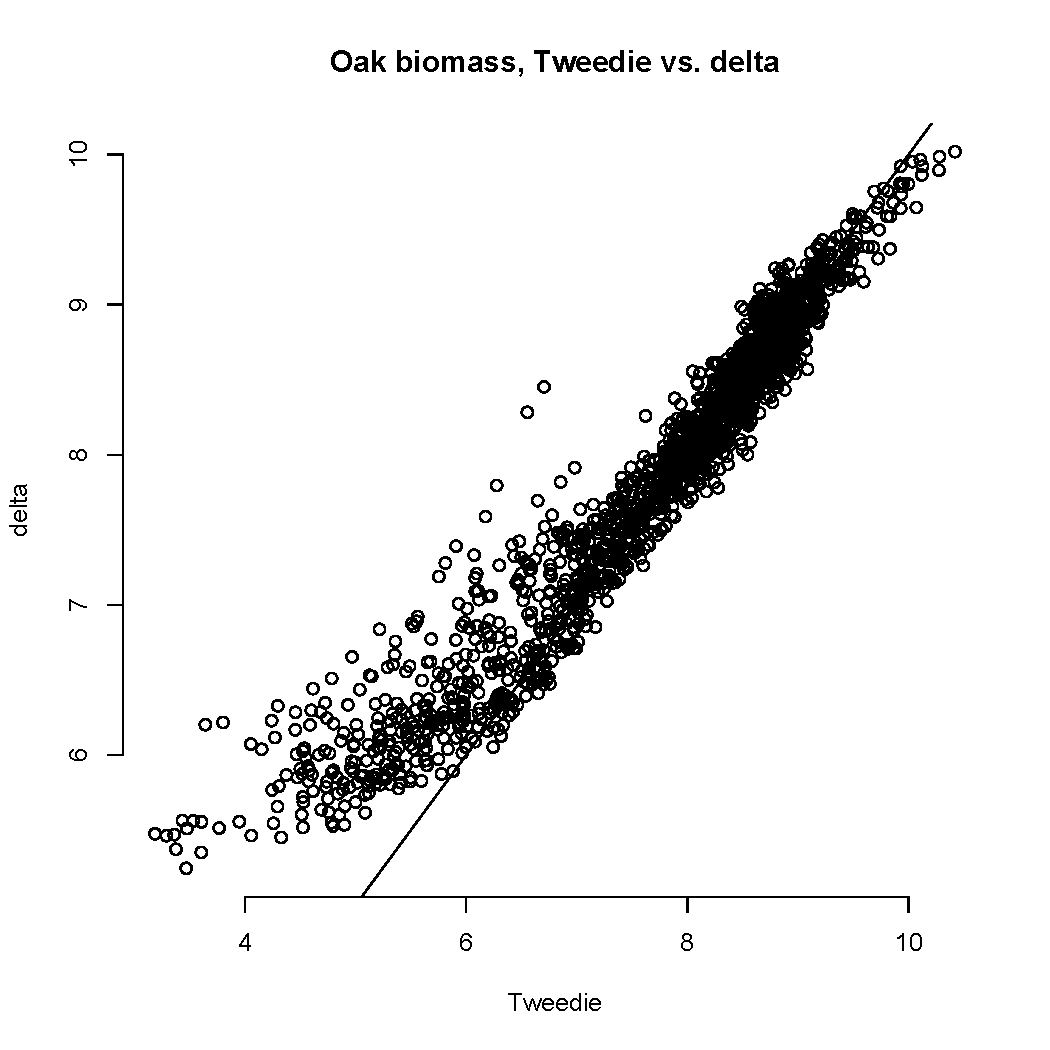
\includegraphics[width=5in]{../../figures/Exploration/Oak-biomass-tweedie2-v-delta.pdf}
	\caption{\label{fig:oaks-biomass-spline}}
	\end{center}
\end{figure}

\begin{figure}
	\begin{center}
	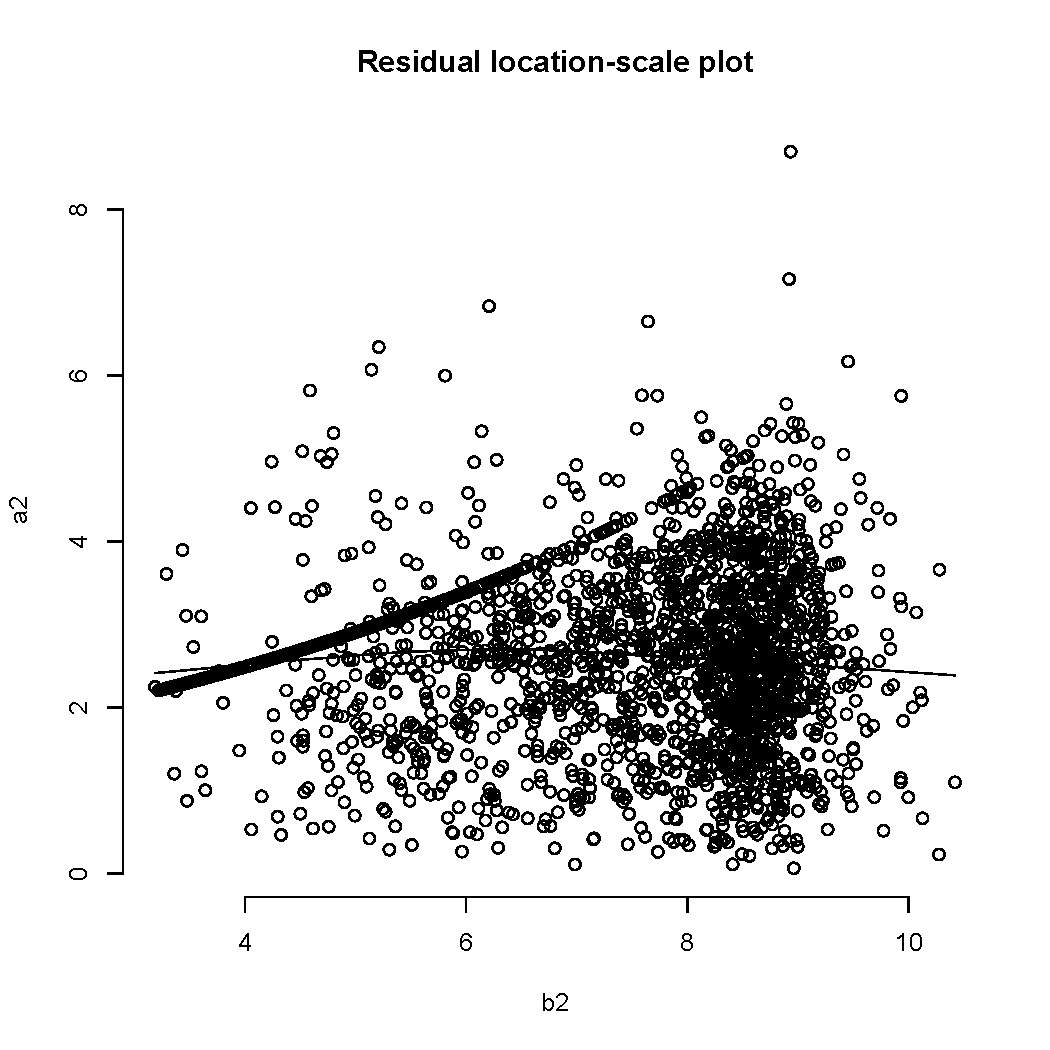
\includegraphics[width=5in]{../../figures/Exploration/Oak-Tweedie2-location-scale.pdf}
	\caption{\label{fig:oaks-tweedie2-location-scale}}
	\end{center}
\end{figure}


\section{References}
%\bibliographystyle{chicago}
%\bibliography{../../references/biomass}

\end{document}  